\section*{2.3 Simple Variational Inference}

\begin{tcolorbox}
\textbf{Question 2.3.9:}
Implement the VI algorithm for the variational distribution in Equation (10.24) in Bishop.
\end{tcolorbox}

The following problem is stated in Bishop. Given a data set $D = \{x_1,...,x_N\}$ of observed values $x$ that are drawn from a Gaussian distribution we want to infer a posterior distribution using variational inference. The likelihood function is given by
\begin{align*}
  p(D|\mu, \tau) = \bigg( \frac{\tau}{2 \pi} \bigg)^{N/2} \text{exp} \bigg\{ - \frac{\tau}{2} \sum_{n=1}^N (x_n-\mu)^2 \bigg\}
\end{align*}
The conjugate prior distributions for $\mu$ and $\tau$ are given by
\begin{align*}
  p(\mu|\tau) & = \mathcal{N} \big( \mu;\mu_0, (\lambda_0\tau)^{-1} \big) \\
  p(\tau) & = \Gamma(\tau;a_0, b_0)
\end{align*}
where $\mu_0, \lambda_0, a_0, b_0$ are hyperparameters. The factorised variational approximation of the posterior is given by
\begin{align*}
  q(\mu, \tau) = q{_\mu}(\mu)q_{\tau}(\tau)
\end{align*}

The factorised distributions are computed in Bishop and become
\begin{align*}
  q{_\mu}(\mu) & = \mathcal{N}(\mu;\mu_N, \lambda_N^{-1}) \\
  q_{\tau}(\tau) & = \Gamma(\tau; a_N, b_N)
\end{align*}
whom are accompanied by the following updating formulas for the parameters. 
\begin{align}
  \mu_N & = \frac{\lambda_0 \mu_0 + N \overline{x}}{\lambda_0 + N}\\
  \lambda_N & = (\lambda_0 + N)\mathbb{E}_{\tau}[\tau] = (\lambda_0 + N) \frac{a_N}{b_N}\\
  a_N & = a_0 + \frac{N}{2} \\
  b_N & = b_0 + \frac{1}{2} \mathbb{E}_{\mu}\Bigg[ \sum_{n=1}^N (x_n - \mu)^2 + \lambda_0 (\mu - \mu_0)^2 \Bigg] \nonumber\\
  & = b_0 + \frac{1}{2} \Bigg[ \sum_{n=1}^N x_n^2 + N \mathbb{E}_{\mu}[\mu^2] - 2N\overline{x}\mathbb{E}_{\mu}[\mu]
          + \lambda_0(\mathbb{E}_{\mu}[\mu^2] + \mu_0^2 - 2\mu_0 \mathbb{E}_{\mu}[\mu]) \Bigg] \nonumber \\
  & = \bigg \{ \mathbb{E}_{\mu}[\mu] = \mu_N , \, \mathbb{E}_{\mu}[\mu^2] = V_{\mu}(\mu) + \mathbb{E}_{\mu}[\mu]^2 = \lambda^{-1} + \mu_N^2 \bigg \} \nonumber \\
  & = b_0 + \frac{1}{2} \Bigg[ \sum_{n=1}^N x_n^2 + (N + \lambda_0)(\lambda^{-1} + \mu_N^2) - 2\mu_N(N\overline{x} + \mu_0 \lambda_0)
          + \lambda_0 \mu_0^2 \Bigg]
\end{align}
The VI algorithm is then implemented by updating the parameters in the order of the equations given above.

\begin{tcolorbox}
\textbf{Question 2.3.10:}
What is the exact posterior?
\end{tcolorbox}
The exact posterior can be computed using the likelihood of the data and the priors. Since the two priors for $\mu$ and $\tau$ are conjugate priors to the likelihood we know that the posterior will be on the form of a Gaussian-Gamma distribution.

\begin{align}
  p(\mu,\tau|D) & \propto  p(D|\mu, \tau)p(\mu|\tau) p(\tau) \nonumber \\
  & \propto \tau^{\frac{N}{2}}\tau^{\frac{1}{2}}\tau^{a_0 - 1} e^{-b_0\tau} \text{exp} \Bigg\{ -\frac{\tau}{2}\Bigg[ \sum_{n=1}^N (x_n - \mu)^2 + \lambda_0 (\mu - \mu_0)^2 \Bigg] \Bigg \} \nonumber \\
  & \propto \tau^{\frac{N}{2}}\tau^{\frac{1}{2}}\tau^{a_0 - 1} e^{-b_0\tau} \text{exp}
   \Bigg\{ -\frac{1}{2}\tau (N + \lambda_0) \bigg( \mu -  \frac{N \overline{x} + \lambda_0 \mu_0}{N \lambda_0} \bigg)^2 \Bigg \} \times \nonumber \\
  & \qquad \text{exp} \Bigg\{ -\frac{\tau}{2}\Bigg[- \frac{(N\overline{x} + \lambda_0\mu_0)^2}{N+\lambda_0} + \sum_{n=1}^N x_n^2 + \lambda_0\mu_0^2 \Bigg] \Bigg \} \nonumber \\
  & \propto \tau^{\frac{N}{2}}\tau^{a_0 - 1} e^{-b_0\tau} \mathcal{N} \bigg( \mu; \frac{N \overline{x} + \lambda_0 \mu_0}{N \lambda_0}, \frac{1}{\tau (N + \lambda_0)} \bigg) \times \nonumber \\
  & \qquad \text{exp} \Bigg\{ -\frac{\tau}{2}\Bigg[- \frac{(N\overline{x} + \lambda_0\mu_0)^2}{N+\lambda_0} + \sum_{n=1}^N x_n^2 + \lambda_0\mu_0^2 \Bigg] \Bigg\} \nonumber \\
  & \propto \mathcal{N} \bigg( \mu; \frac{N \overline{x} + \lambda_0 \mu_0}{N \lambda_0}, \frac{1}{\tau (N + \lambda_0)} \bigg) \times \nonumber \\
  & \qquad \Gamma \bigg(\tau; a_0 + \frac{N}{2},
  b_0 + \frac{1}{2}\big (\sum_{n=1}^N x_n^2 + \lambda_0 \mu_0^2 - \frac{(N\overline{x} + \lambda_0\mu_0)^2}{N+\lambda_0}\big ) \bigg)
  \label{exact_posterior}
\end{align}
The exact posterior is thus given by the expression in equation (\ref{exact_posterior}) where $\Gamma(\tau; \alpha, \beta)$ denotes the gamma distribution with shape $\alpha$ and rate $\beta$ as parameters.
\\

\begin{tcolorbox}
\textbf{Question 2.3.11:}
Compare the inferred variational distribution with the exact posterior. Run the inference on data points drawn from iid Gaussians. Do this for three interesting cases and visualize the results. Describe the differences.
\end{tcolorbox}
The following plots were obtained when comparing the inferred posterior to the real posterior.


\begin{figure}[H]
  \centering
  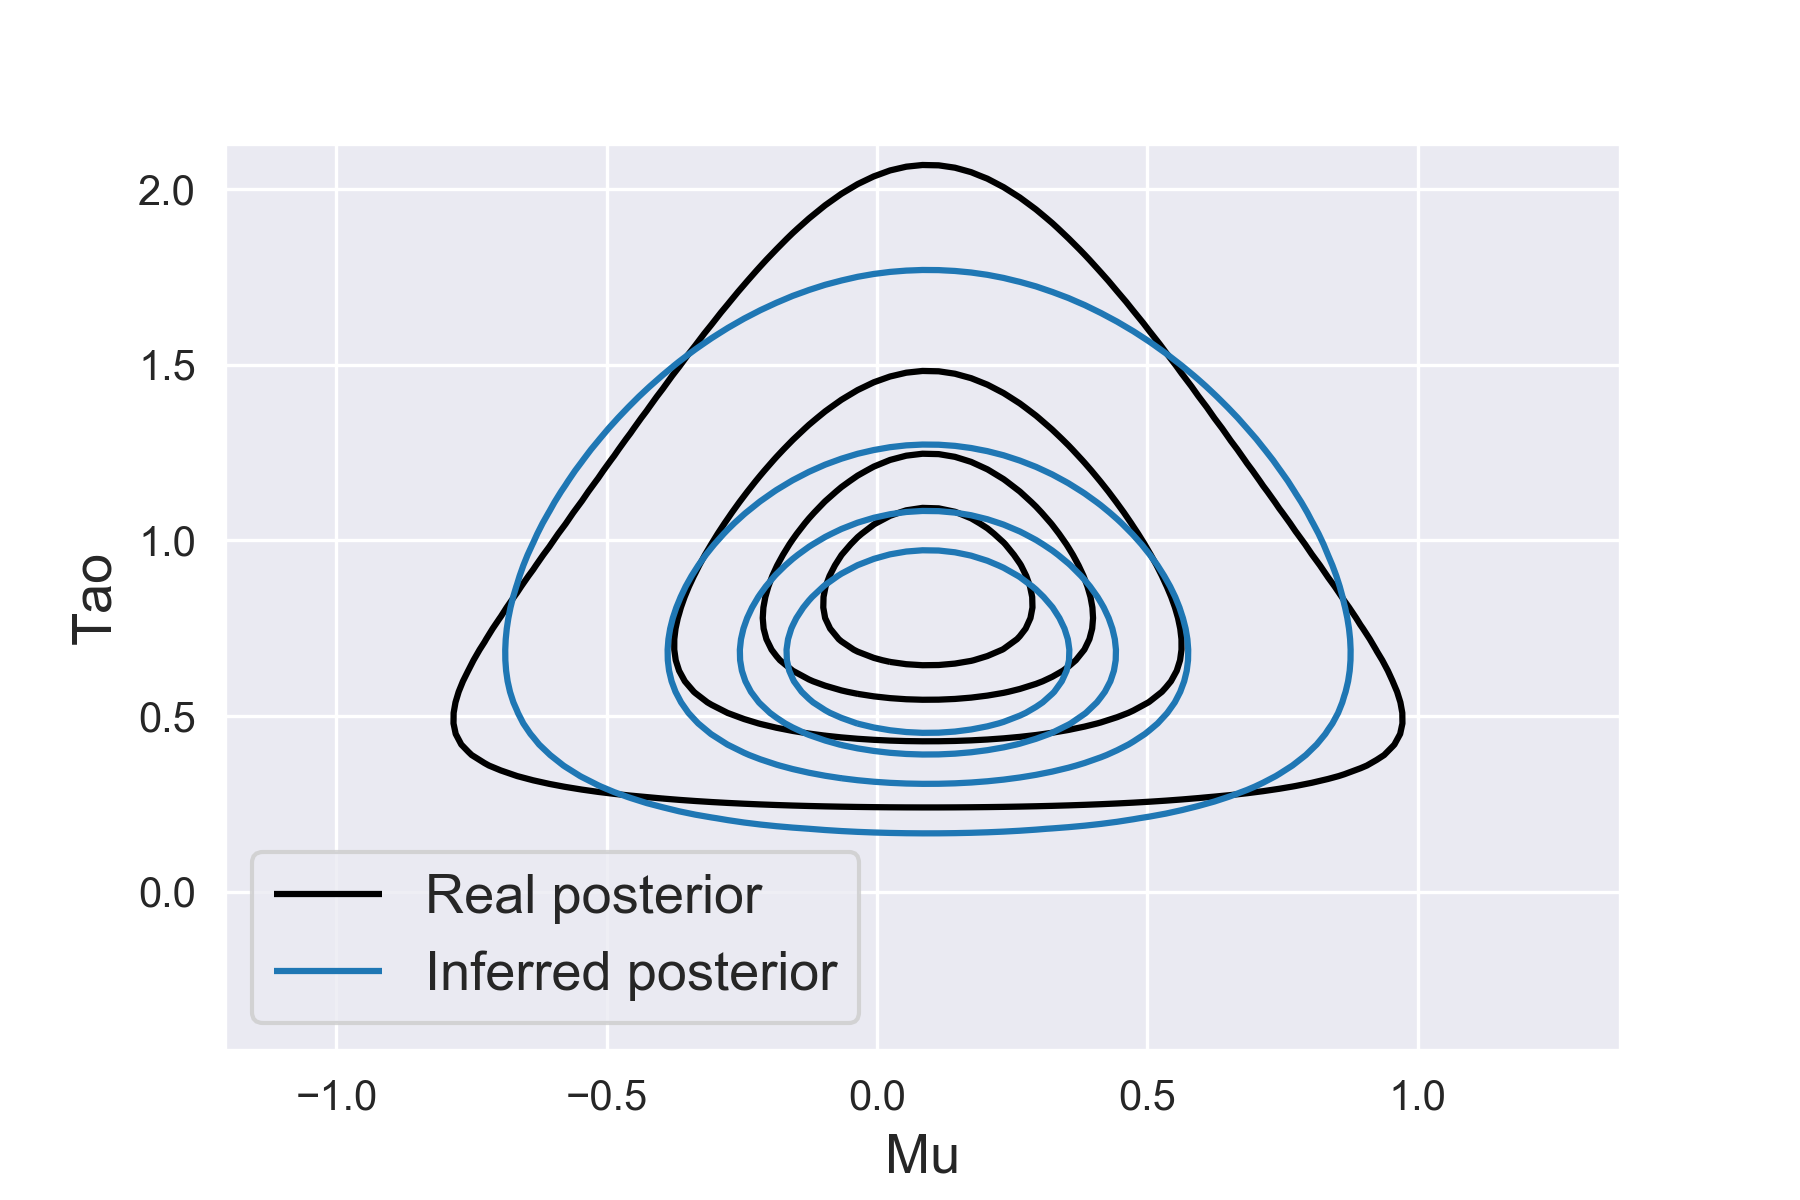
\includegraphics[width=\linewidth]{VI_plot_N_10-mu_0-tau_1.png}
  \caption{10 data points drawn from $\mathcal{N}(0,1)$, all hyperparameters set to $0$}
  \label{VI_1}
\end{figure}

In Figure \ref{VI_1} one can see a similar behaviour to the book as the hyperparameters are set the same. The real target for the parameters are $(\mu, \tau) = (0,1)$ which the real posterior seem to be a bit closer to but considering the low number of data points both distributions perform quite well. When comparing the shape of the the two posteriors one can see that the real posterior is closer to a triangle than the inferred posterior but in general the inferred posterior is close to the real posterior. Note that the uncertainty is about the same for both $\mu$ and $\tau$.

\begin{figure}[H]
  \centering
  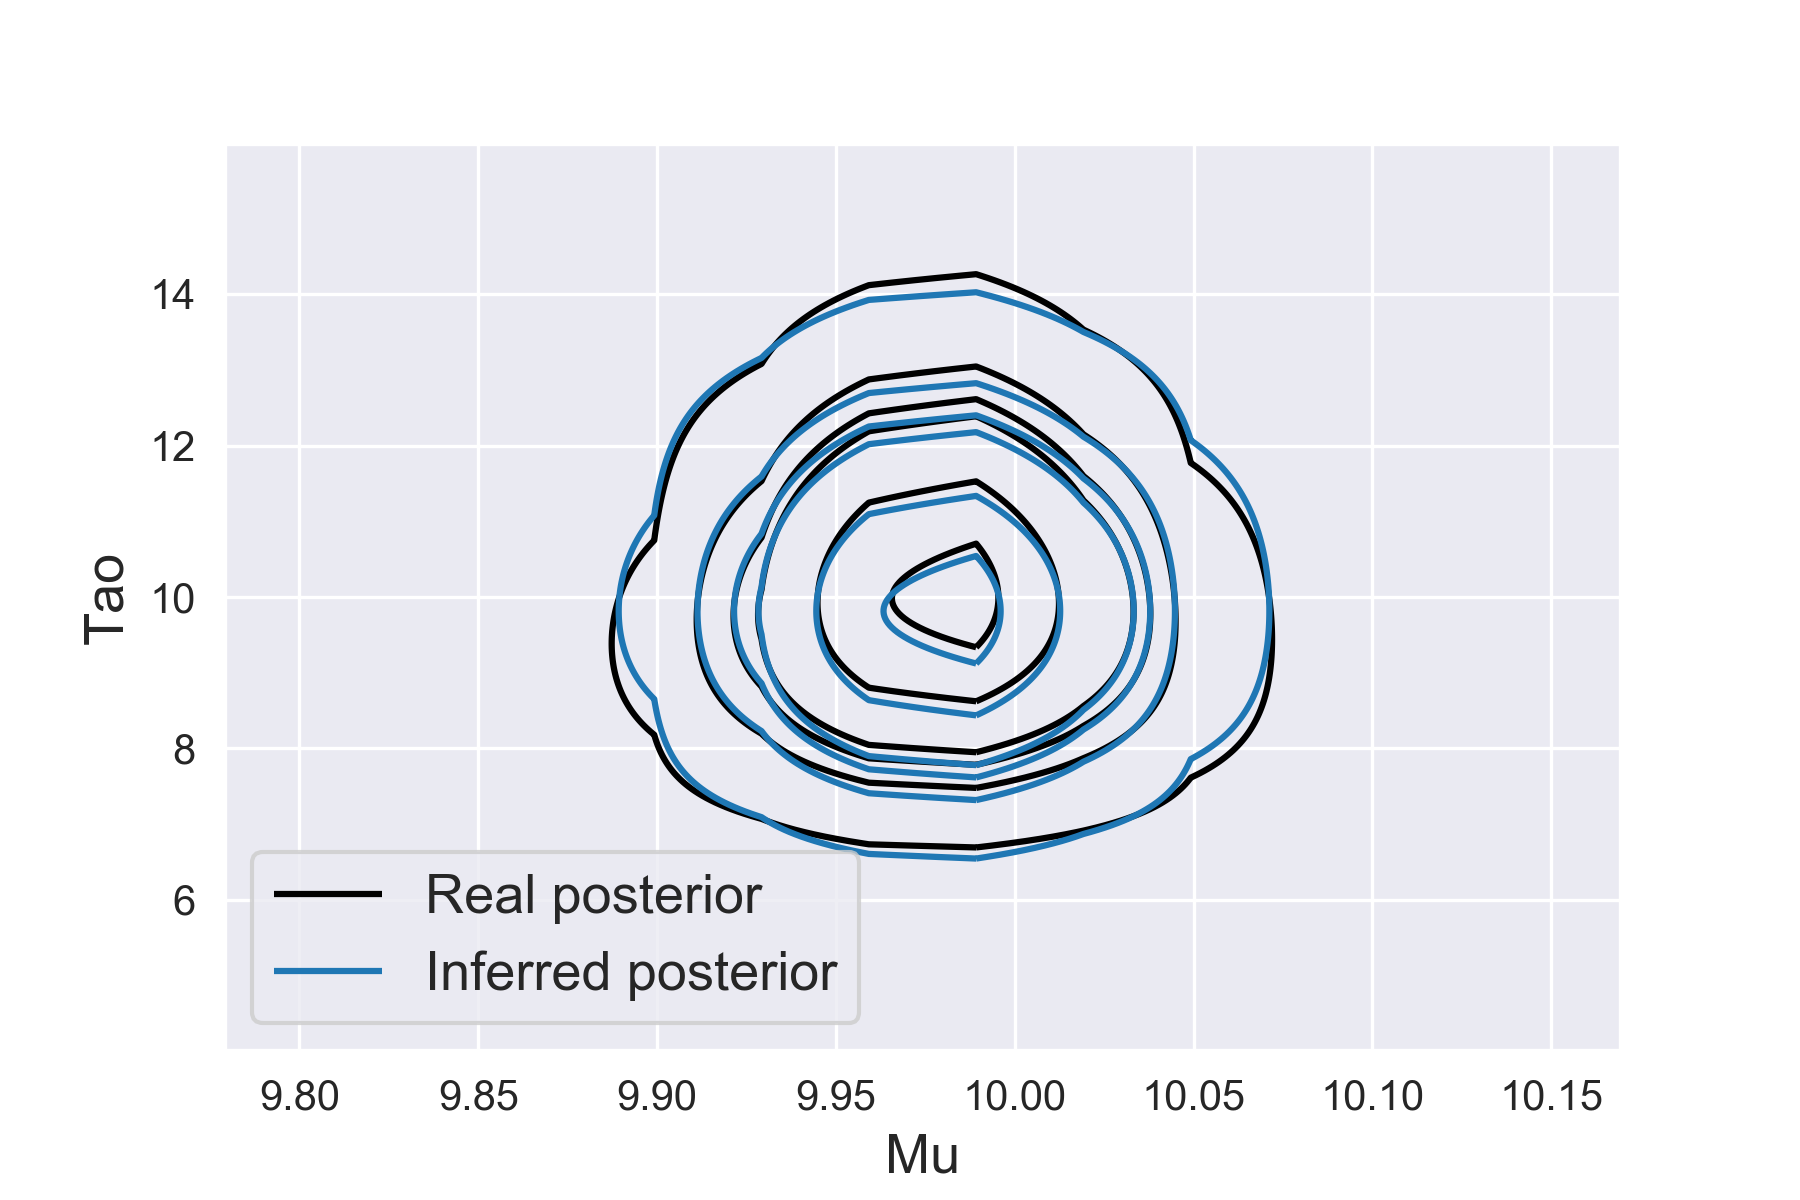
\includegraphics[width=\linewidth]{VI_plot_N_100-mu_10-tau_10.png}
  \caption{100 data points drawn from $\mathcal{N}(10,\frac{1}{10})$, all hyperparameters set to $0$}
  \label{VI_2}
\end{figure}
In Figure \ref{VI_2} the number of data points has increased to $100$ and the distribution they are generated from has changed to $\mathcal{N}(10,\frac{1}{10})$. Noticing that the axis scales are different here the conclusions from Figure \ref{VI_1} still holds except that the uncertainty in $\tau$ is almost two orders of magnitude larger than the uncertainty for $\mu$.

\begin{figure}[H]
  \centering
  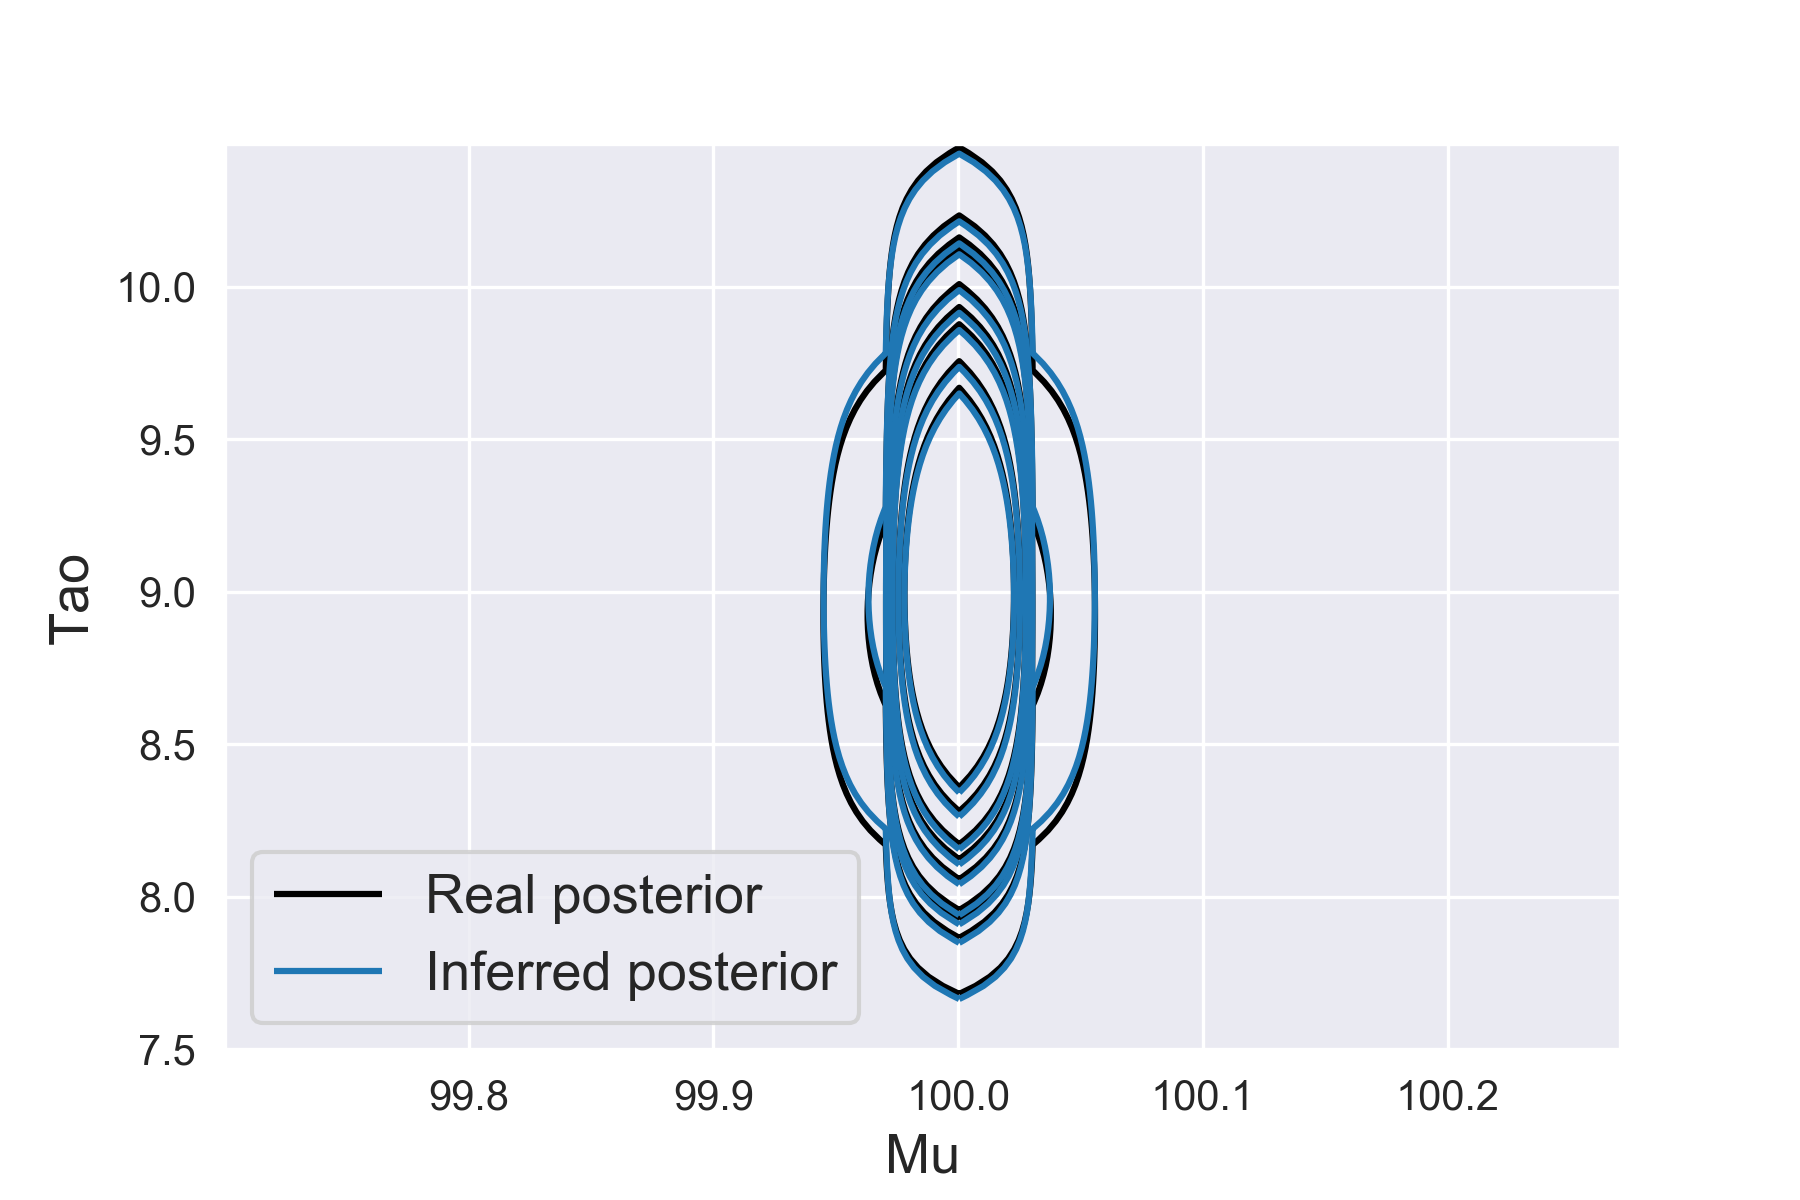
\includegraphics[width=\linewidth]{VI_plot_N_1000-mu_100-tau_100.png}
  \caption{1000 data points drawn from $\mathcal{N}(100,\frac{1}{100})$, all hyperparameters set to $0$}
  \label{VI_3}
\end{figure}

\begin{figure}[H]
  \centering
  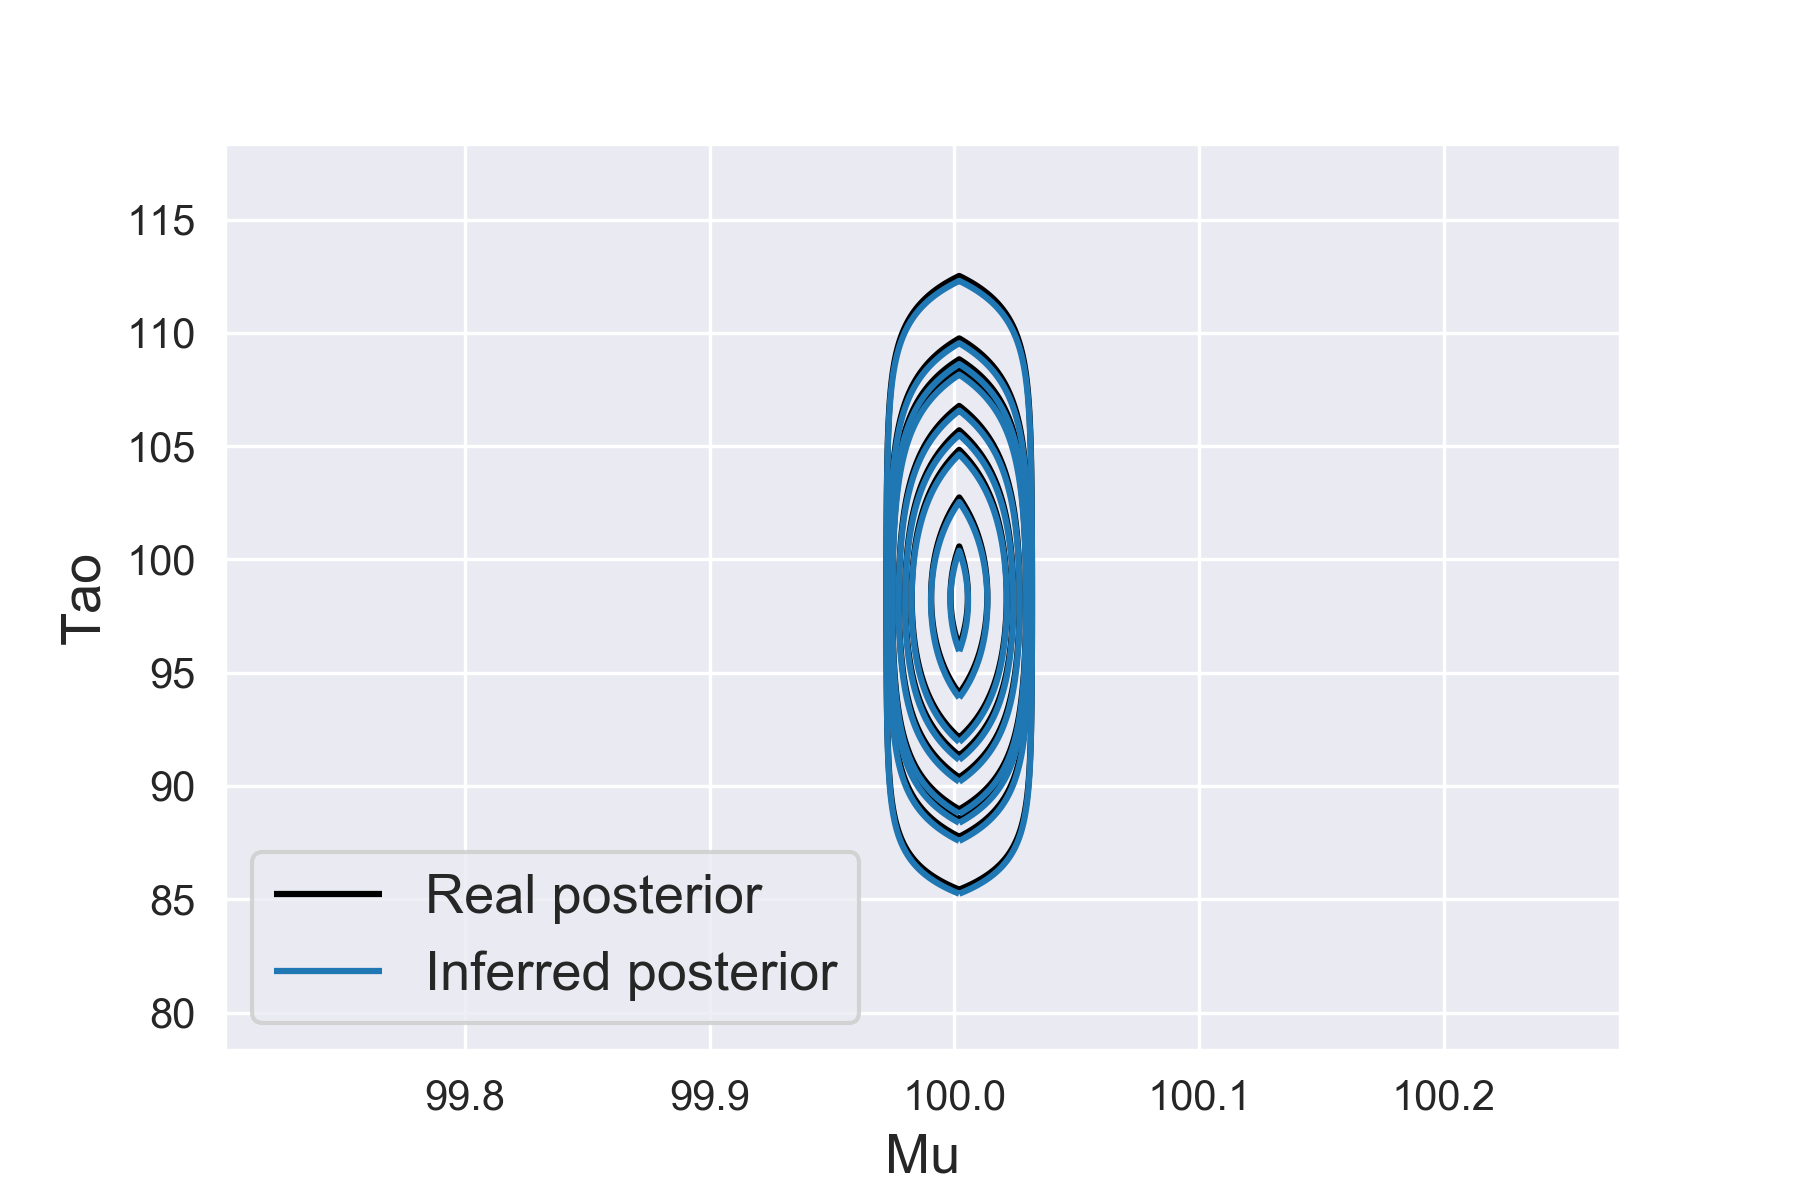
\includegraphics[width=\linewidth]{VI_plot_N_1000-mu_100-tau_100-mu0_100.png}
  \caption{1000 data points drawn from $\mathcal{N}(100,\frac{1}{100})$, all hyperparameters set to $0$ except $\mu_0 = 100$ }
  \label{VI_4}
\end{figure}

In Figures \ref{VI_3} and \ref{VI_4} the effect of the hyperparameter $\mu_0$ is enlightened. In both examples $1000$ data points are drawn from $\mathcal{N}(100,\frac{1}{100})$. In Figure \ref{VI_3} when $\mu_0 = 0$ both posteriors are centred around $\tau = 9$, very far from the real value of $\tau = 100$ whilst in Figure \ref{VI_4} both posteriors are centred around $\tau = 98$, very close to the real value. This shows how important the hyperparameters can be if one does not have a sufficient amount of data. In addition to this conclusion one can also conclude that the inferred posterior is very similar to the real posterior in this example.
